% -*- coding: utf-8 -*-
\documentclass[10pt,serif,t]{beamer}
\usepackage{times}
\usepackage[T1]{fontenc}
\usepackage{fancybox}
\usepackage{amsthm}
\usepackage{amsmath}
\usepackage{amsfonts}
\usepackage{graphicx}
\usepackage{subfigure}
\usepackage[adobefonts]{ctex} 

\usedictionary{basic}
\uselanguage{SimplifiedChinese}
\languagepath{SimplifiedChinese}
\setbeamertemplate{caption}[numbered]
%% \renewcommand{\proofname}{证明}

\usetheme{Madrid}

\newcommand*{\ket}[1]{\left\vert{#1}\right\rangle}
\newcommand{\cell}[3]{\parbox[c][#2][c]{#1}{\makebox[#1]{#3}}} 

\title{\heiti{}测试beamer文档类的简体中文翻译}
\author{\songti{}胡海星}
\institute{\kaishu{}计算机科学与技术系\\
           南京大学}
\date{\today}

\begin{document}
%%%%%%%%%%%%%%%%%%%%%%%%%%%%%%%%%%%%%%%%%%%%%%%%%%%%%%%%%%%%%%%%%%%%%%%%%%%%%%%

\begin{frame}
    \titlepage
\end{frame}

\begin{frame}
  \frametitle{目录}
  \tableofcontents
\end{frame}

\section{第一节}

\subsection{第一小节}

\begin{frame}
  \frametitle{测试定理环境}
  \begin{theorem}
    测试测试测试测试测试测试测试测试测试测试测试测试测试测试测试测试,
    测试测试测试测试测试测试测试测试测试测试。测试测试测试测试测试测试,
    测试测试测试测试测试测试测试测试。
  \end{theorem}
  \begin{proof}
    证明证明证明证明证明证明证明,证明证明证明证明证明证明证明。证明证明证明证明,
    证明证明证明证明证明证明证明。
  \end{proof}
\end{frame}

\subsection{第二小节}

\begin{frame}
  \frametitle{测试引理环境}
  \begin{lemma}
    测试测试测试测试测试测试测试测试测试测试测试测试测试测试测试测试,
    测试测试测试测试测试测试测试测试测试测试。测试测试测试测试测试测试,
    测试测试测试测试测试测试测试测试。
  \end{lemma}
  \begin{proof}
    证明证明证明证明证明证明证明,证明证明证明证明证明证明证明。证明证明证明证明,
    证明证明证明证明证明证明证明。
  \end{proof}
\end{frame}

\section{第二节}

\subsection{第一小节}

\begin{frame}
  \frametitle{测试例子环境}
  \begin{example}
    测试测试测试测试测试测试测试测试测试测试测试测试测试测试测试测试,
    测试测试测试测试测试测试测试测试测试测试。测试测试测试测试测试测试,
    测试测试测试测试测试测试测试测试。
  \end{example}
\end{frame}

\subsection{第二小节}

\begin{frame}
  \frametitle{测试推论环境}
  \begin{corollary}
    测试测试测试测试测试测试测试测试测试测试测试测试测试测试测试测试,
    测试测试测试测试测试测试测试测试测试测试。测试测试测试测试测试测试,
    测试测试测试测试测试测试测试测试。
  \end{corollary}
\end{frame}

\section{第三节}

\subsection{第一小节}

\begin{frame}
  \frametitle{测试定义环境}
  \begin{definition}
    测试测试测试测试测试测试测试测试测试测试测试测试测试测试测试测试,
    测试测试测试测试测试测试测试测试测试测试。测试测试测试测试测试测试,
    测试测试测试测试测试测试测试测试。
  \end{definition}
\end{frame}

\subsection{第二小节}

\begin{frame}
  \frametitle{测试事实环境}
  \begin{fact}
    测试测试测试测试测试测试测试测试测试测试测试测试测试测试测试测试,
    测试测试测试测试测试测试测试测试测试测试。测试测试测试测试测试测试,
    测试测试测试测试测试测试测试测试。
  \end{fact}
\end{frame}

\begin{frame}
  \frametitle{测试定义环境}
  \begin{definition}
    测试测试测试测试测试测试测试测试测试测试测试测试测试测试测试测试,
    测试测试测试测试测试测试测试测试测试测试。测试测试测试测试测试测试,
    测试测试测试测试测试测试测试测试。
  \end{definition}
\end{frame}

\begin{frame}
  \frametitle{测试插图}  
  \begin{figure}
    \centering
    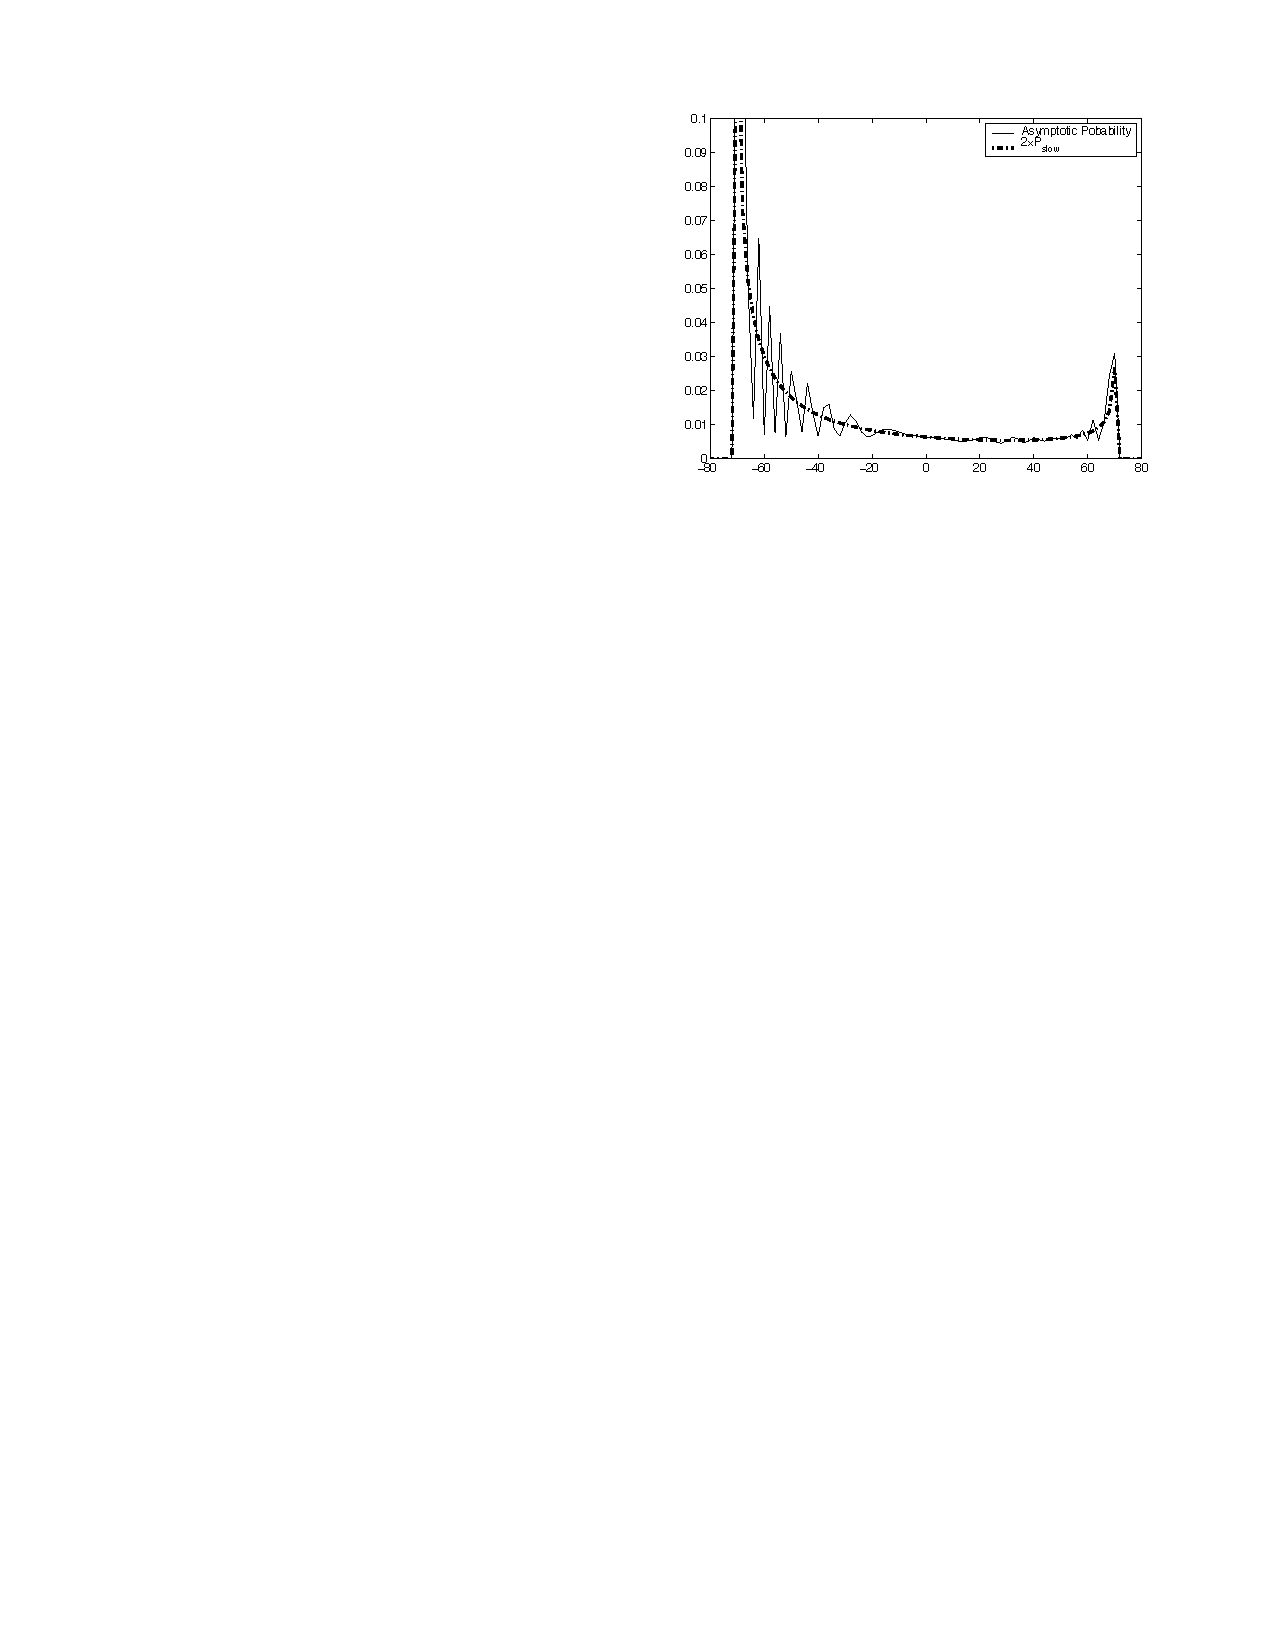
\includegraphics[height=0.6\textheight]{1d_hadamard_quantum_walk.pdf}
    \caption{一维离散Hadamard量子游走位置状态概率分布}
  \end{figure}
\end{frame}

\begin{frame}
  \frametitle{测试表格}  
\begin{table}
    \centering
  	\begin{tabular}{|c||c|c|c|c|c|c|c|c|c|c|c|}
    \hline
      \cell{1em}{1em}{$n$} 
    & \cell{1em}{1em}{$-5$} 
    & \cell{1em}{1em}{$-4$} 
    & \cell{1em}{1em}{$-3$} 
    & \cell{1em}{1em}{$-2$}
    & \cell{1em}{1em}{$-1$}
    & \cell{1em}{1em}{$0$}
    & \cell{1em}{1em}{$1$} 
    & \cell{1em}{1em}{$2$} 
    & \cell{1em}{1em}{$3$} 
    & \cell{1em}{1em}{$3$} 
    & \cell{1em}{1em}{$5$} \\ 
    \hline
      $0$ & & & & & & $1$ & & & & & \\ 
    \hline	
      $1$ & & & & & $\frac{1}{2}$ & & $\frac{1}{2}$ & & & & \\ 
    \hline
      $2$ & & & & $\frac{1}{4}$  & & $\frac{2}{4}$ & & $\frac{1}{4}$ & & & \\ 
    \hline
      $3$ & & & $\frac{1}{8}$ & & $\frac{5}{8}$ & & $\frac{1}{8}$ & & $\frac{1}{8}$ & & \\ 
    \hline
      $4$ & & $\frac{1}{16}$ & & $\frac{10}{16}$ & & $\frac{2}{16}$ & & $\frac{2}{16}$ & & $\frac{1}{16}$ & \\ 
    \hline
      $5$ & $\frac{1}{32}$ & & $\frac{17}{32}$ & & $\frac{4}{32}$ & & $\frac{4}{32}$& & $\frac{5}{32}$ & & $\frac{1}{32}$ \\    
    \hline
  	\end{tabular}
    \caption{一维离散Hadamard量子游走经过$5$步后的位置状态概率分布}
	\end{table} 
\end{frame}

%%%%%%%%%%%%%%%%%%%%%%%%%%%%%%%%%%%%%%%%%%%%%%%%%%%%%%%%%%%%%%%%%%%%%%%%%%%%%%%
\end{document}
